%% It is just an empty TeX file.
%% Write your code here.
\chapter{Communication System Test}



\section {ParSec Communication System}
Various signals transmitted in industrial environment have different requirements in terms of dependability. Let's consider a simple CCTV video transmission system. Each frame, even in low resolution solutions, consists of several hundred thousands pixels. The frame rate lies somewhere between 30 and 5 frames per second, depending on the requirements. Even multiple bit error in the compressed video information bitstream leads just to the corruption of some frames. Depending on the error rate and frame rate, such disturbance may not influence the correct service at all, just lowering the video quality. The system, despite some errors, still fulfills it's function. 
On the other hand the information flow between the control system and the nodes, placed on the robotic arms on the assembly line, consists in constant transmission of the coordinates of the destination and position of the arm. An error in such information can lead to the damage of manipulated objects or another catastrophic system failure.
Moreover, the quality of the signal propagation in such a rapidly changing environment is not constant. The error rate can significantly rise for a short time, but be relatively low otherwise. Spending time, power and resources on complex encoding and decoding may not be justified for the majority of the systems life time. The ability to adapt to the quality of the transmission would be just another advantage of well designed communication system.
In conclusion, the requirements of the industrial wireless system are diversified and need a configurable solution, that could offer a constantly high level of dependability while adapting to its environment and the use case. The high level of dependability means the coverage of the hardware faults in the first place, since they can even prevent the establishment and synchronization of the connection.

The goal of the ParSec project is to create a dependable, flexible and secure wireless communication system which meets all industrial automation requirements. It has to work with latencies below 1 ms and with very high noise level, serving many distributed clients at once. Moreover it has to deal with fading effects and potentially many reflections or even obstacles coming in the way of transmission and breaking it.

The ParSec communication system (shown in~\autoref{fig:ParSec}) consists of the MAC Layer processing, taking place within a standard processor, implemented mostly as software routines. The standard industrial bus, where all instructions come from. Followed by the FEC unit and by a frame formatter. The last part is the baseband processor, which consists of mixed and analog signal processing and Radio Frequency unit. 

\begin{figure}[h]
\centering
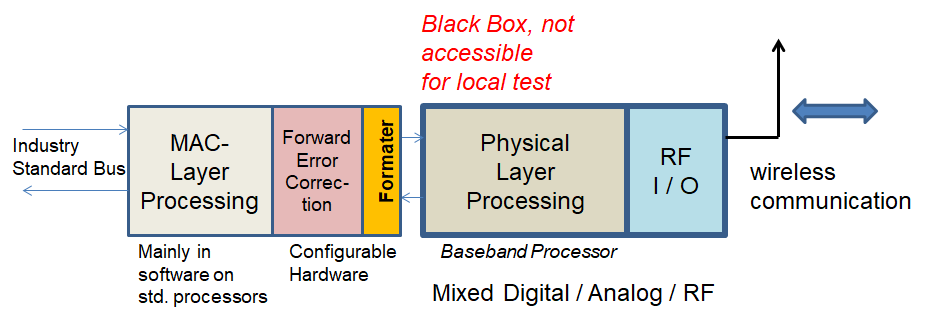
\includegraphics[width=0.65\textwidth]{figures/ParSec.png}
\caption{Block Diagram of the ParSec communiaction system}
\label{fig:ParSec}
\end{figure}

The dependability of such a system is threatened by many factors:
\begin{itemize}
    \item random errors in the noisy channel and soft errors due to transient faults in hardware modules
    \item hard errors due to permanent faults in hardware modules
\end{itemize}

\subsection{FEC in ParSec project}
laying between FEC encoder and decoder, can be indivisible corrected thanks to ECC, as long as their number doesn't exceed the ECC correction capability\cite{source}. There are many techniques to improve the signal quality and make it resistant to fading effects due to multi-path signal propagation, poor signal-to-noise ratio or interferences, lowering the error rate. The known and used techniques involve Orthogonal Frequency Domain Multiplexing (OFDM) \cite{book:OFDM,art:OFDM}, Spread-Spectrum Communication \cite{art:spread-spectrum96,art:spread-spectrum97} or Ultra Wide-Band Frequency Communication \cite{book:ultra-wide08,book:ultra-wide04}. The ParSec project has to face environments even worse then anticipated during creation of those methods and with much shorter latencies. The OFDM technique would be suitable, but it needs many very fast AD converters~\cite{art:PSSS04}. The solution chosen for ParSec is Parallel Sequence Spread Spectrum (PSSS) technology~\cite{art:PSSS15,art:PSSS04,patent}. It provides comparable transmission quality as OFDM, without the cost of expensive AD converters.

hard errors due to permanent faults in hardware modules require special treatment since they can even prevent the synchronization of transceiver and receiver and therefore cannot be so easily corrected by FEC. Since permanent faults don't disappear, they also need special repair mechanism, which often means a doubling of the unit or its parts. The fault diagnosis proves to be complicated, especially in the mixed signal and analog parts, moreover when the access to this parts is limited. When an IP is shipped as a "black box" and there is no possibility to implement any internal DfT techniques, some sort of external test is required. 



\section{Functional Shorts Concept}
Thanks to ECC, a precise detection of error positions in the received bitstream is possible, as long as the error count doesn't exceed its correcting capabilities. The idea behind the diagnostic test based on extended FEC functions is to use the existing FEC redundancy and detect not only soft errors and transmission errors, but also hard errors. As mentioned in the~\autoref{sub:limits} the ECC can be used in hardware monitoring only if the input and output of the UUT are identical. Since the wireless communication is usually a duplex communication, every node happens to own both, the transmitter and receiver. They consist of complementary building blocks. Every modulator in transmitter is substituted with a demodulator in receiver, every encoder with decoder. The basic task of the receiver modules is to recreate the original information sent by transmitter, step by step, layer by layer. A diagnostic test would require to short the transmitter with receiver and systematically short the outputs of every module with the inputs of their corresponding module. With encoder and decoder in one closed system, it should be possible to detect the exact positions of errors in the bitstream and identify faulty units. The decoder would act as a response analyzer. In this way, the information leaving FEC encoder arrives at the input of FEC decoder, manipulated only by permanent faults in the shorted modules. The idea is presented in~\autoref{fig:Shorts}. 

\begin{figure}[h]
\centering
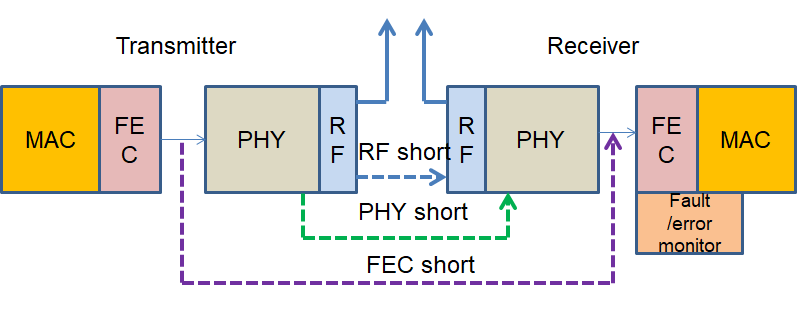
\includegraphics[width=0.65\textwidth]{figures/Shorts.png}
\caption{Transmitter and receiver shortcut idea for diagnostic test purposes}
\label{fig:Shorts}
\end{figure}

In order to conclude such test, the physical shorts need to be implemented. A simple multplexer demultiplexer pair with the common control logic would allow to choose between a normal functionality and shortened path. Additionally the test vectors need to be generated or stored in ROM. The fault detection occurs thanks to an extended decoder functionality, which signalizes, with a special ISERR output, if the current bit of the bit stream has been flipped or not. This functionality is also used during the normal data flow, to adjust the transmission parameters and adapt the FEC algorithm. A simple counter connected to this special output counts the number of bit flips in every block. This information can be used for channel quality estimation. 
The idea of functional shorts has been implemented into the Test Bench together with fault injection capability and is shown in \autoref{fig:shorts_ena}. The injected fault vector manipulates the output of any chosen module to simulate the possible effects of hardware faults on the processed information. The implementation lacks real modules, except from the encoder and decoder. Every other module is implemented as a simple delay in the digital information flow. The Air simulates the communication channel. 

\begin{figure}[h]
\centering
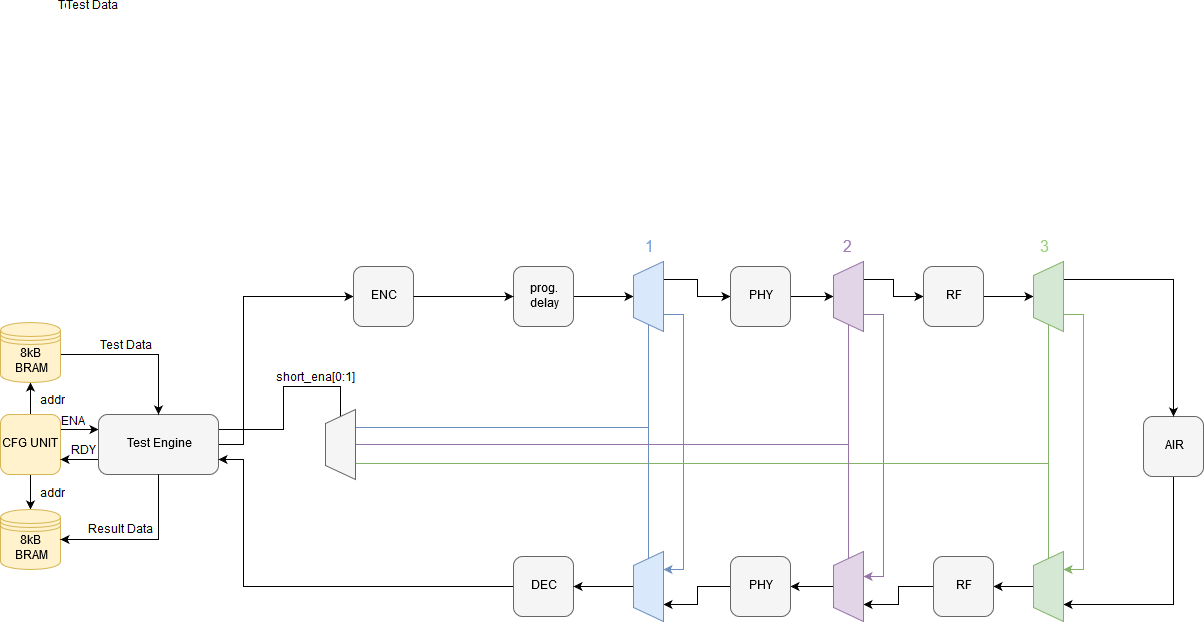
\includegraphics[width=0.65\textwidth]{figures/Short_ena.png}
\caption{Implementation of functional shorts into the Test Bench}
\label{fig:short_ena}
\end{figure}

\subsection{Diagnostic test Procedure}
Let's assume, that the FEC decoder is fault-free and that every module owns some sort of repair ability. The erroneous unit would be the Radio Frequency unit of the receiver.
\begin{enumerate}
    \item Start the test by enabling the shortcut nr. 3, closing the test loop between transmitter and receiver
    \item Conclude the test by running all test vectors through the design, placing them on the inputs of FEC encoder, until the first occurrence of the ISERR set high
    \item Enable shortcut nr. 2
    \item Run test again and detect no errors, since the faulty unit is not in the test loop
    \item Run repair procedure on the transmitter RF unit
    \item Enable Shortcut nr. 2
    \item Run the test only to see the ISERR is high again
    \item Run repair procedure on RF unit of the receiver, revert the repair of the transmitter RF unit
    \item Start the test again to see no errors detected
\end{enumerate}

The diagnostic test efficiency is only as good as the FEC implementation. Let's try to examine the encoder and decoder to see what are the limitations of the procedure and what kinds of faults and in what number can be detected.

\section{Test of BCH(1023,943) Encoder}
The Programmable Encoder Architecture (PENCA) designed by P. Pfeifer, firstly introduced in \ref{art:Pfeifer}, used within the ParSec project, contains an internal test capability. 
\section{Test of BCH(1023,943) Decoder}
\section{Test of transmission path with known average error rate}
The Unit Under Test consists of one chosen, hard coded BCH(1023,943) encoder capable of correcting up to 8 bits per block. The decoder is followed by simple XOR gate, which overlays encoder output with error vector, simulating random errors in transmission path and transient errors in data processing digital logic laying on-path. The last module is the corresponding BCH decoder, with output indicating if the next data bit has been repaired or not. All modules are separated by flip-flops to simulate the delay that happens on the way between encoder and decoder. The error vector is supplied as just another input of the Test Bench.\\

The test starts with issuing the reset signal for one clock cycle, that will be propagated firstly to the encoder and later to the decoder input. The primary data input consists of $t$ randomly generated test vectors of length 943, followed by zeros to tact out the system response. The error vector has to be generated with care, to assure the exact average weight of all vectors and induce errors only within the block length. All error vectors are generated as one long vector with first $f_c$ bits set to one and rest to zero. The length of the vector is equal to $t\times n$, where $n=1023$ is the length of a packet. The error vector is randomly permuted and split into $n$ vectors. As a result the exact number of errors is normally distributed throughout all error vectors. The error vectors are shifted into the system along with input data, resulting in controlled corruption of encoder output. The erroneous data arrives at the decoder inputs one clock cycle after the reset and gets processed 97 tacts before valid data appears on the data output. Every test creates an independent run, so the data is not chained one after another, on the contrary, it is shifted with zeros out. So after shifting in the 943 data bits, there are 80 consecutive zeros for the parity, 2 zeros for the delay between encoder and decoder, 97 zeros for decoder calculations and 943 zeros to shift out the decoder response. There is also one additional zero at the beginning due to the reset signal. All together every test vector consists of $l=1+943+80+2+97+943=2066b$. The test was built with 1000 test vectors for each error number, starting from 1 error per packet and ending with 12.5, with step 0.5; giving the overall of 24000 tests. The version of the Test Engine used was configured as 8 input, so although not all inputs are used, the full description of one clock cycle takes 1 byte. It gives around $2kB$ (for each test) and $48MB$ (for all tests) of data, that has to be shifted through a hardware module.

Prior to the test, few simulations were conducted, in order to see how many packets contain more errors $f_c$ than the code is able to correct. The simulation summed only the number of errors in each packet and compared it with the code capability, giving the number of packets that should not be able to pass the test. The test was suppose to validate, if the hardware modules give the same statistic of failed tests and therefore failed packets by known average error rate. For each test new randomization was conducted. The result is shown in~\autoref{fig:realsim}.

\begin{figure}[h]
\centering
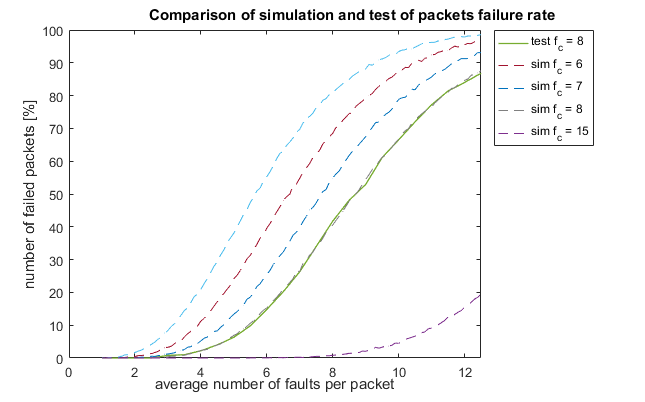
\includegraphics[width=0.7\textwidth]{figures/real+simulated.png}
\caption{}
\label{fig:realsim}
\end{figure}

The test result is showed as continuous line and is compliant with the simulation result. Moreover it can be noticed, that despite the high number of 8 errors that a code can correct, a dependable (error-free) transfer of 1000 packets could be observed only for 2.5 errors per packet. For 3.5 errors per packet, already 1\% of all packets failed. For 8 errors it is already 40\% of failed transfers. The most dependable solution for now, used in PENCA, is capable of correcting 15 bit errors in one packet, which is indicated as a violet dashed line in~\autoref{fig:realsim}.\\

All those tests assume that only random errors, both in hardware and during wireless transmission pose threat against a communication system. The deterioration of hardware leads also to hard errors due to permanent faults. Th influence of permanent faults on error correcting capabilities of ECC has been illustrated in~\autoref{fig:simperm}.

\begin{figure}[h]
\centering
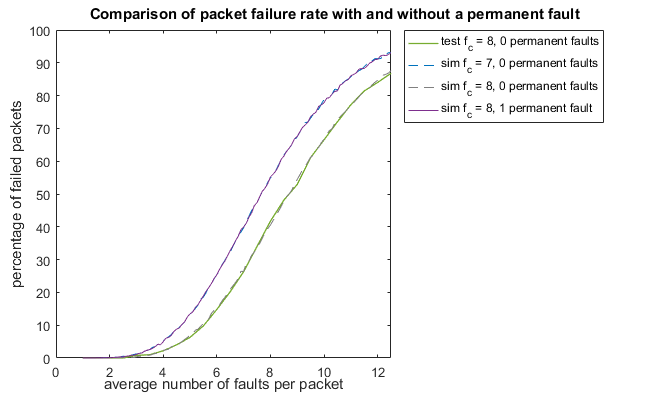
\includegraphics[width=0.7\textwidth]{figures/simulated+perm.png}
\caption{}
\label{fig:simperm}
\end{figure}

The permanent fault is modeled as stack-at-one-fault resulting in a single bit error in data stream. Additionally the average number of errors was induced to simulate an ongoing communication. The resulting curve reveals, that in the presence of a permanent fault the code capability is diminished by a number of errors that this fault produces. A code with correcting capability of 8 errors per packet behaves like a code, with 7 errors correcting capability. The permanent faults pose one additional threat, which is not obvious at the first glance. The FEC works only for a stable synchronized communication system, that is already running. A permanent fault may prevent the creation of stable communication link between transmitter and receiver. Even with the most dependable codes, if the information doesn't reach the channel decoder, all FEC redundancy becomes useless.

\section{Test in presence of permanent faults}\label{sec:shorts}
General implementation of FEC covers only some of possible errors, namely: transient faults in hardware and in the wireless signal propagation channel, but only under the condition of synchronized and stable communication path. Faults in modules, required for the synchronization process, both transient and permanent, need to be taken care of differently. pose As described here~\autoref{art:Gleichner}, 
All modules of the communication system come in pairs that are complementary to each other. The demodulators task is to recreate the possible codeword \textbf{v} from the waveform received from the RF module. The same codeword that the modulator has translated into waveform in the transmitter. The waveform arriving at the receiver should match with the one sent by the transmitter (in ideal noiseless system). The channel decoder takes the code word and recreates the information sequence \textbf{u\^}, which previously entered the channel encoder. The signals, although maybe altered by transmission error or hardware error, should have the same form. The interface of each corresponding module of the receiver is an exact copy of the one placed in the transmitter, only exactly in the opposite direction. This ability can be used later for test purposes, excluding some modules from the communication path and feeding the corresponding modules with their pairs output directly.
If there was a possibility to exclude the noisy channel from the communication path, then all detected errors would have to have they origin within the hardware modules, indicating the presence of permanent faults. Such test could happed periodically or during the systems start up.
To implement such solution the transmitter would have to be directly connected with the receiver. Since communication modules are usually designed for both: transmitting and receiving, and all of their components come in complementary pairs, it would be possible to connect the outputs of transmitter modules to corresponding inputs of receivers modules. The idea of such "functional shorts" is shown in \autoref{fig:shorts}.
\subsection{System Partitioning for Test}
Another aspect of dependable communication systems is the wireless connection itself and the modulation used to provide the maximal insensitivity to multi-path propagation problems, fading effects and frequency interferences. The state-of-the art solutions incorporate Orthogonal Frequency Domain Multiplexing (OFDM) \ref{OFDM}, spread-spectrum communication \ref{spread-spectrum} or ultra wide-band frequency communication \ref{ultra wide-band}...
PSSS, 
 As mentioned in \autoref{sub:testa} the testability of mixed signal and analog components is limited at best or requires instrumentation. 
